\documentclass[../Main.tex]{subfiles}

\begin{document}
    \subsection{Overview}
        This is an exploration game, where you explore a randomised maze collecting items and followers on your way to help defeat the monsters, while also trying to find the escape route - which will be a room with a trapdoor.
    \subsection{Maze Generation}
        \subsubsection{Maze Needed}
            My plan for the maze is for it for it to be infinite, meaning that it only generates part of the maze at a time, and as you explore, you uncover more of the maze. However, for memory efficiency, the maze that is no longer loaded, won't be stored in memory and so deleted.
        \subsubsection{Types}
            There is both labyrinths and mazes. Labyrinths have only one path. This means that there is minimal choice in where the user can decide to go.
            The other type is mazes. These are multicursal, meaning it has multiple paths. This allows the user to choose their own path.
        \subsubsection{Approaches to Generation}
            \begin{itemize}
                \item Cellular Automation Algorithm

                This is based on John Conway's Game of Life, where a cell is created if it has exactly 3 neighbours and can survive it has 1-5 neighbors. However, this means that with the same starting pattern, the same maze will be created everytime.

                \item Prim's Algorithm

                This is where a random point on the maze is chosen as the starting point. Then all the surrounding areas are added to a list. Then the program continually generates new sections and adds more areas to the list, until the list is completely empty and all the spaces on the board is taken up. The positives with this is that it creates a randomised maze everytime, that takes up the whole map. However, the disadvantage is that when generating more sections, the maze cannot go back on itself.
            \end{itemize}
        \subsubsection{Conclusion}
            In conclusion, to make an infinite maze, I shall be using my own algorithm. This is slightly based off Prim's Algorithm, however instead of filling up the whole board, it leaves gaps. This is done by randomising entrances when placing a cell and then added only those possibilities to the list to generate more. This means that when the player moves north, it is able to generate paths that go back on itself however lead to dead end and not connect back up to the maze. This I feel will make a more dynamic maze when continually exploring the maze.
    \clearpage
    \subsection{Existing Solutions}
        \subsubsection{The Binding of Isaac}
            A similar game is The Binding of Isaac. What I liked about this game was the exploration and randomness, along with the challenge of fighting monsters in different rooms. However, I found it frustrating that there was limiting exploration on each level, as the level is not infinite. Furthermore, another issue I had was the only help that you could get was a familiar, in my game I wish to improve this by having set NPCs that you can find when exploring each level. Also, in binding of Isaac, the scrolling is  not smooth, jumping between each room. Also there are no corridors, making it seem less maze like.
            \begin{figure}[hbt!]
                \centerline{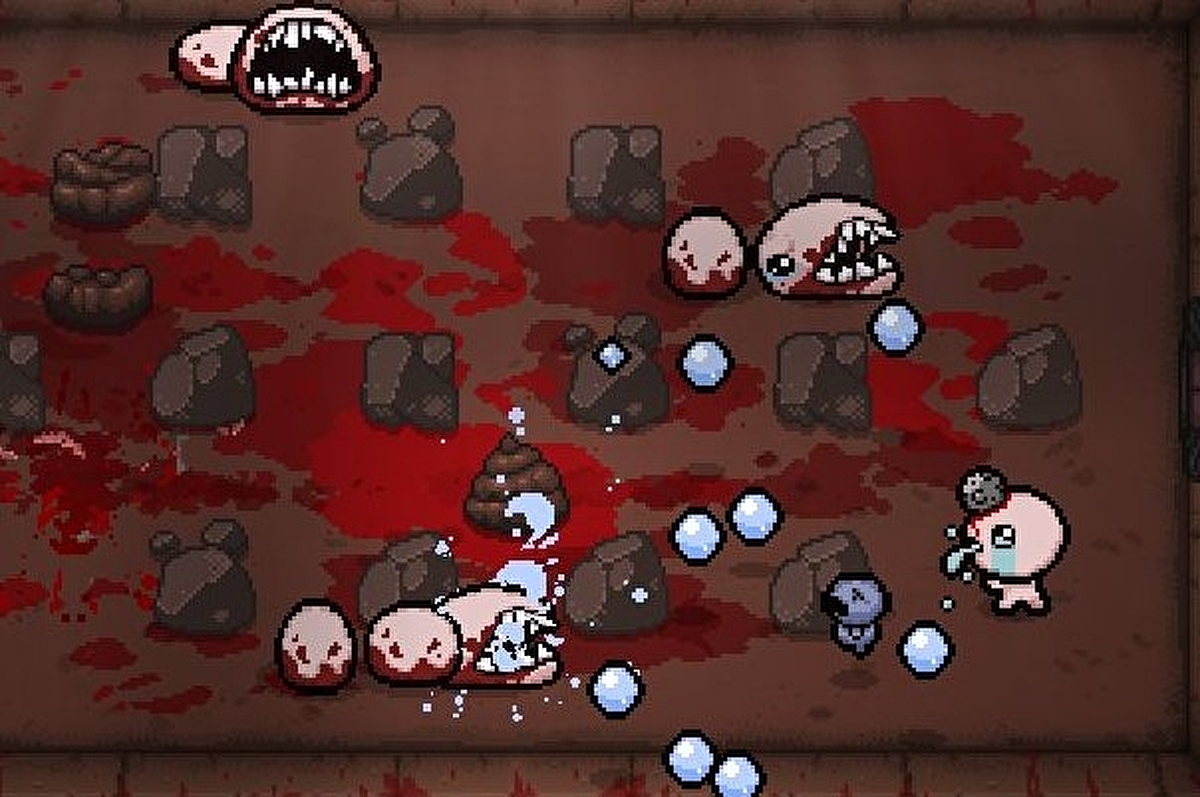
\includegraphics[scale=0.3]{img/The Binding of Isaac.jpg}}
                \caption{Picture from the binding of Isaac, showing the player (bottom right) attacking the enemies}
            \end{figure}
    \clearpage
    \subsection{End Users}
        \subsubsection{\textbf{Description}}
            Teenagers who enjoy exploration video games. They should know the basic mechanics of a video game, such as using W, A, S, D keys to move around and space bar to attack. They should also have a curiosity to explore and play around with what they can do, as this would hopefully make it easier for them to understand how the game works, as the game will not have a tutorial explaining how the game works.
        \subsubsection{Questionnaire}
            \begin{itemize}
                \item Have you played an exploration game before?
                \begin{figure}[hbt!]
                    \centerline{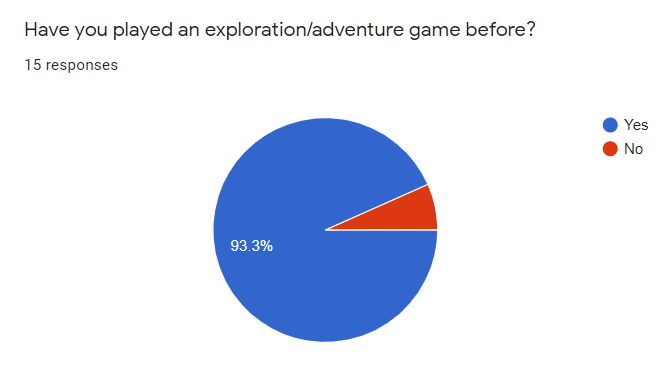
\includegraphics[scale=0.9]{img/Survey/Played Exploration Game.PNG}}
                    \caption{Responses from survey showing most people have played an exploration game}
                    \label{fig:Question1}
                \end{figure}
                % \clearpage
                \item How important is each section when looking for a game?
                \begin{itemize}
                    \item Boss fights
                    \item NPCs that you can interact with
                    \item Enemies that attack you
                    \item Good story
                \end{itemize}
                \begin{figure}[hbt!]
                    \centerline{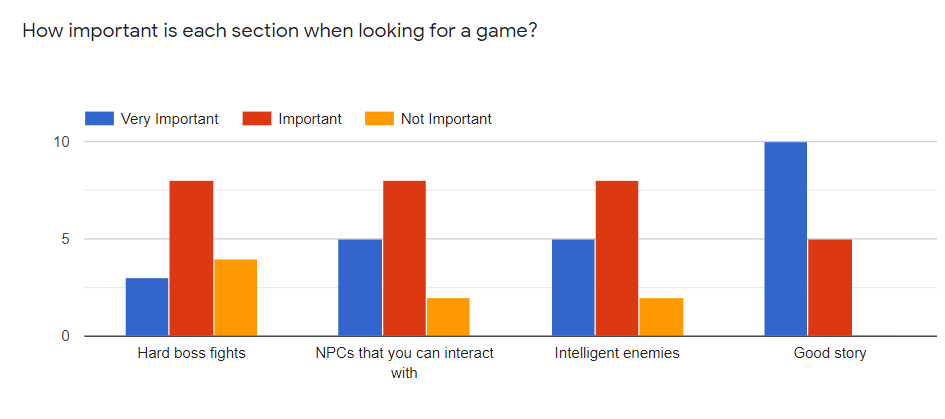
\includegraphics[scale=0.9]{img/Survey/Importance of games.PNG}}
                    \caption{Responses from the story showing that it is equally important to have intelligent enemies and NPCs you can interact with}
                    \label{fig:Question2}
                \end{figure}
                \clearpage
                \item What era do you like games to be designed as?
                \begin{itemize}
                    \item Future
                    \item Modern
                    \item Medieval
                    \item Stone Age
                    \item Multiple eras
                \end{itemize}
                \begin{figure}[hbt!]
                    \centerline{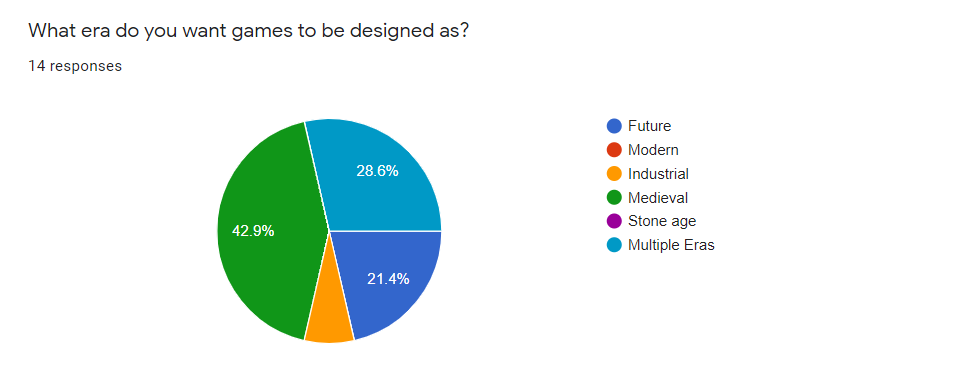
\includegraphics[scale=1]{img/Survey/Era of Games.PNG}}
                    \caption{Responses from survey showing that most people like a Medieval design}
                    \label{fig:Question3}
                \end{figure}
                \item Which do you prefer a weight-based system for the inventory (e.g. in Skyrim) or a space-based system (e.g. Minecraft)?
                \begin{figure}[hbt!]
                    \centerline{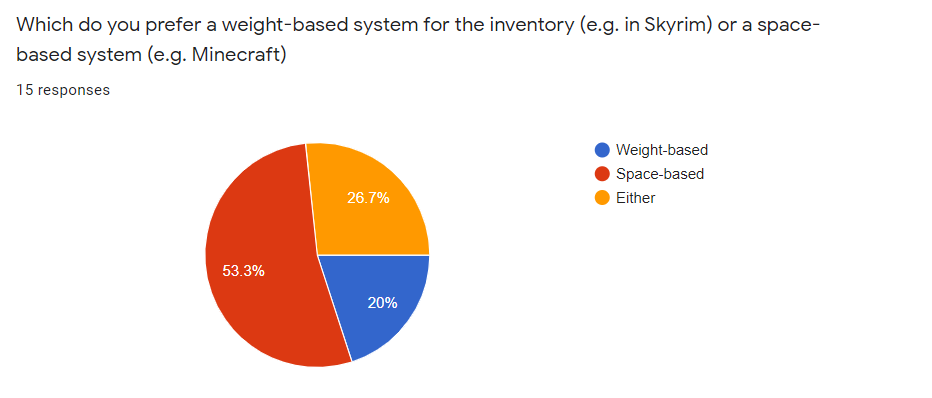
\includegraphics[scale=1]{img/Survey/Inventory system.PNG}}
                    \caption{Responses from survey showing that most people like a weight-based system in a game}
                    \label{fig:Question4}
                \end{figure}
                \clearpage
                \item Do you prefer being able to move while attacking or a Pokémon style attack system?
                \begin{figure}[hbt!]
                    \centerline{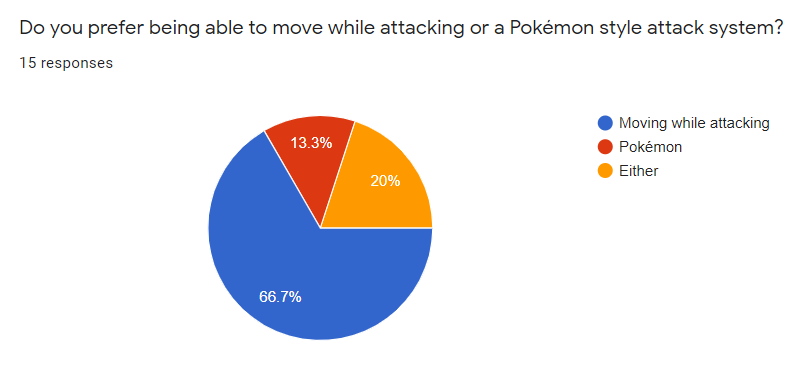
\includegraphics[scale=1]{img/Survey/Attacking System.PNG}}
                    \caption{Responses from survey showing that the attacking system should allow you to still control the player}
                    \label{fig:Question5}
                \end{figure}
                \item Have you played "The Binding of Isaac"?
                \begin{figure}[hbt!]
                    \centerline{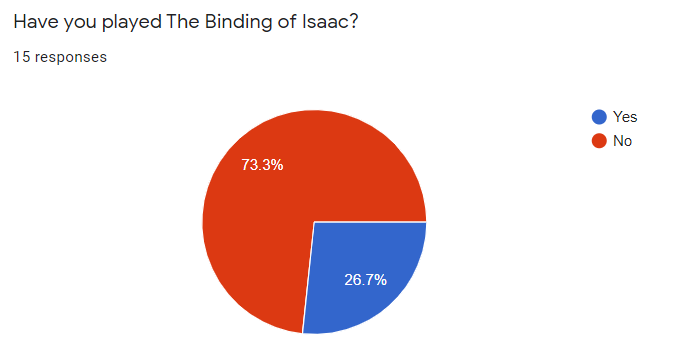
\includegraphics[scale=1]{img/Survey/Capture.PNG}}
                    \caption{Responses from survey showing that most people in this survey had not played The Binding of Isaac}
                    \label{fig:Question6}
                \end{figure}
                \begin{itemize}
                    \item If they had I asked what they liked about the game and what they think could be better (talked about in the conclusion)
                \end{itemize}
            \end{itemize}
            \clearpage
    \subsubsection{Conclusion}
        As shown in \figurename{ 2}, most people taking the survey had played and exploration or adventure game before, this means that the survey would be somewhat respective of the audience this game will be made for. Surprisingly, in \figurename{ 3}, most people believed that hard boss fights are less important than NPCs you can interact with and intelligent enemies, so I will prioritise those features over creating boss fights. For the design, I will be going for a Medieval theme as it seems as though most people prefer that design scheme (as shown in \figurename{ 4}). Also, I have chosen to use a space-based system for the inventory as in \figurename{ 5}, most people responding that they prefer that system. Also, I will allow the player to attack at any point in the maze (for example shooting a projectile) because (as shown in \figurename{ 6}) people prefer it over an attacking GUI.

        As shown in \figurename{ 7}, only a few percentage had played The Binding of Isaac. when asked what they liked about the game, the responses included:
        \begin{itemize}
            \item The rougelike aspect (a subgenre of game that have generated levels, and tile-based graphics)
            \item The replayability and unique style
        \end{itemize}
        Most responses where talking about the rougelike aspect or the randomised levels. From this I have decided to use tile-based graphics with most sprites with a resolution of 64 pixels by 64 pixels to make it more rougelike also I want to make the maze as randomised as possible, meaning that many stats will be randomised.

        % When asked what they would improve about the game, a few people responded saying:
        % \begin{itemize}
        %     \item More routes down
        %     \item A good run is greatly depend on loot found in the first couple of floors.
        % \end{itemize}
        % From this, it seems that the reliance of chance for loot needs to be carefully managed. So, to combat this I have decided to change loot up between the levels, meaning that you cannot get overpowered loot on the first levels. Also I have decided to add a leveling system that allows you to upgrade your stats to allow more ways to play the game. Furthermore, I will need to create multiple ways to get down to different levels, for examples stairs, or a hidden passage that leads you to a treasure room on the next level.
    \clearpage
    \subsection{Structure}
        \begin{figure}[hbt!]
            \centerline{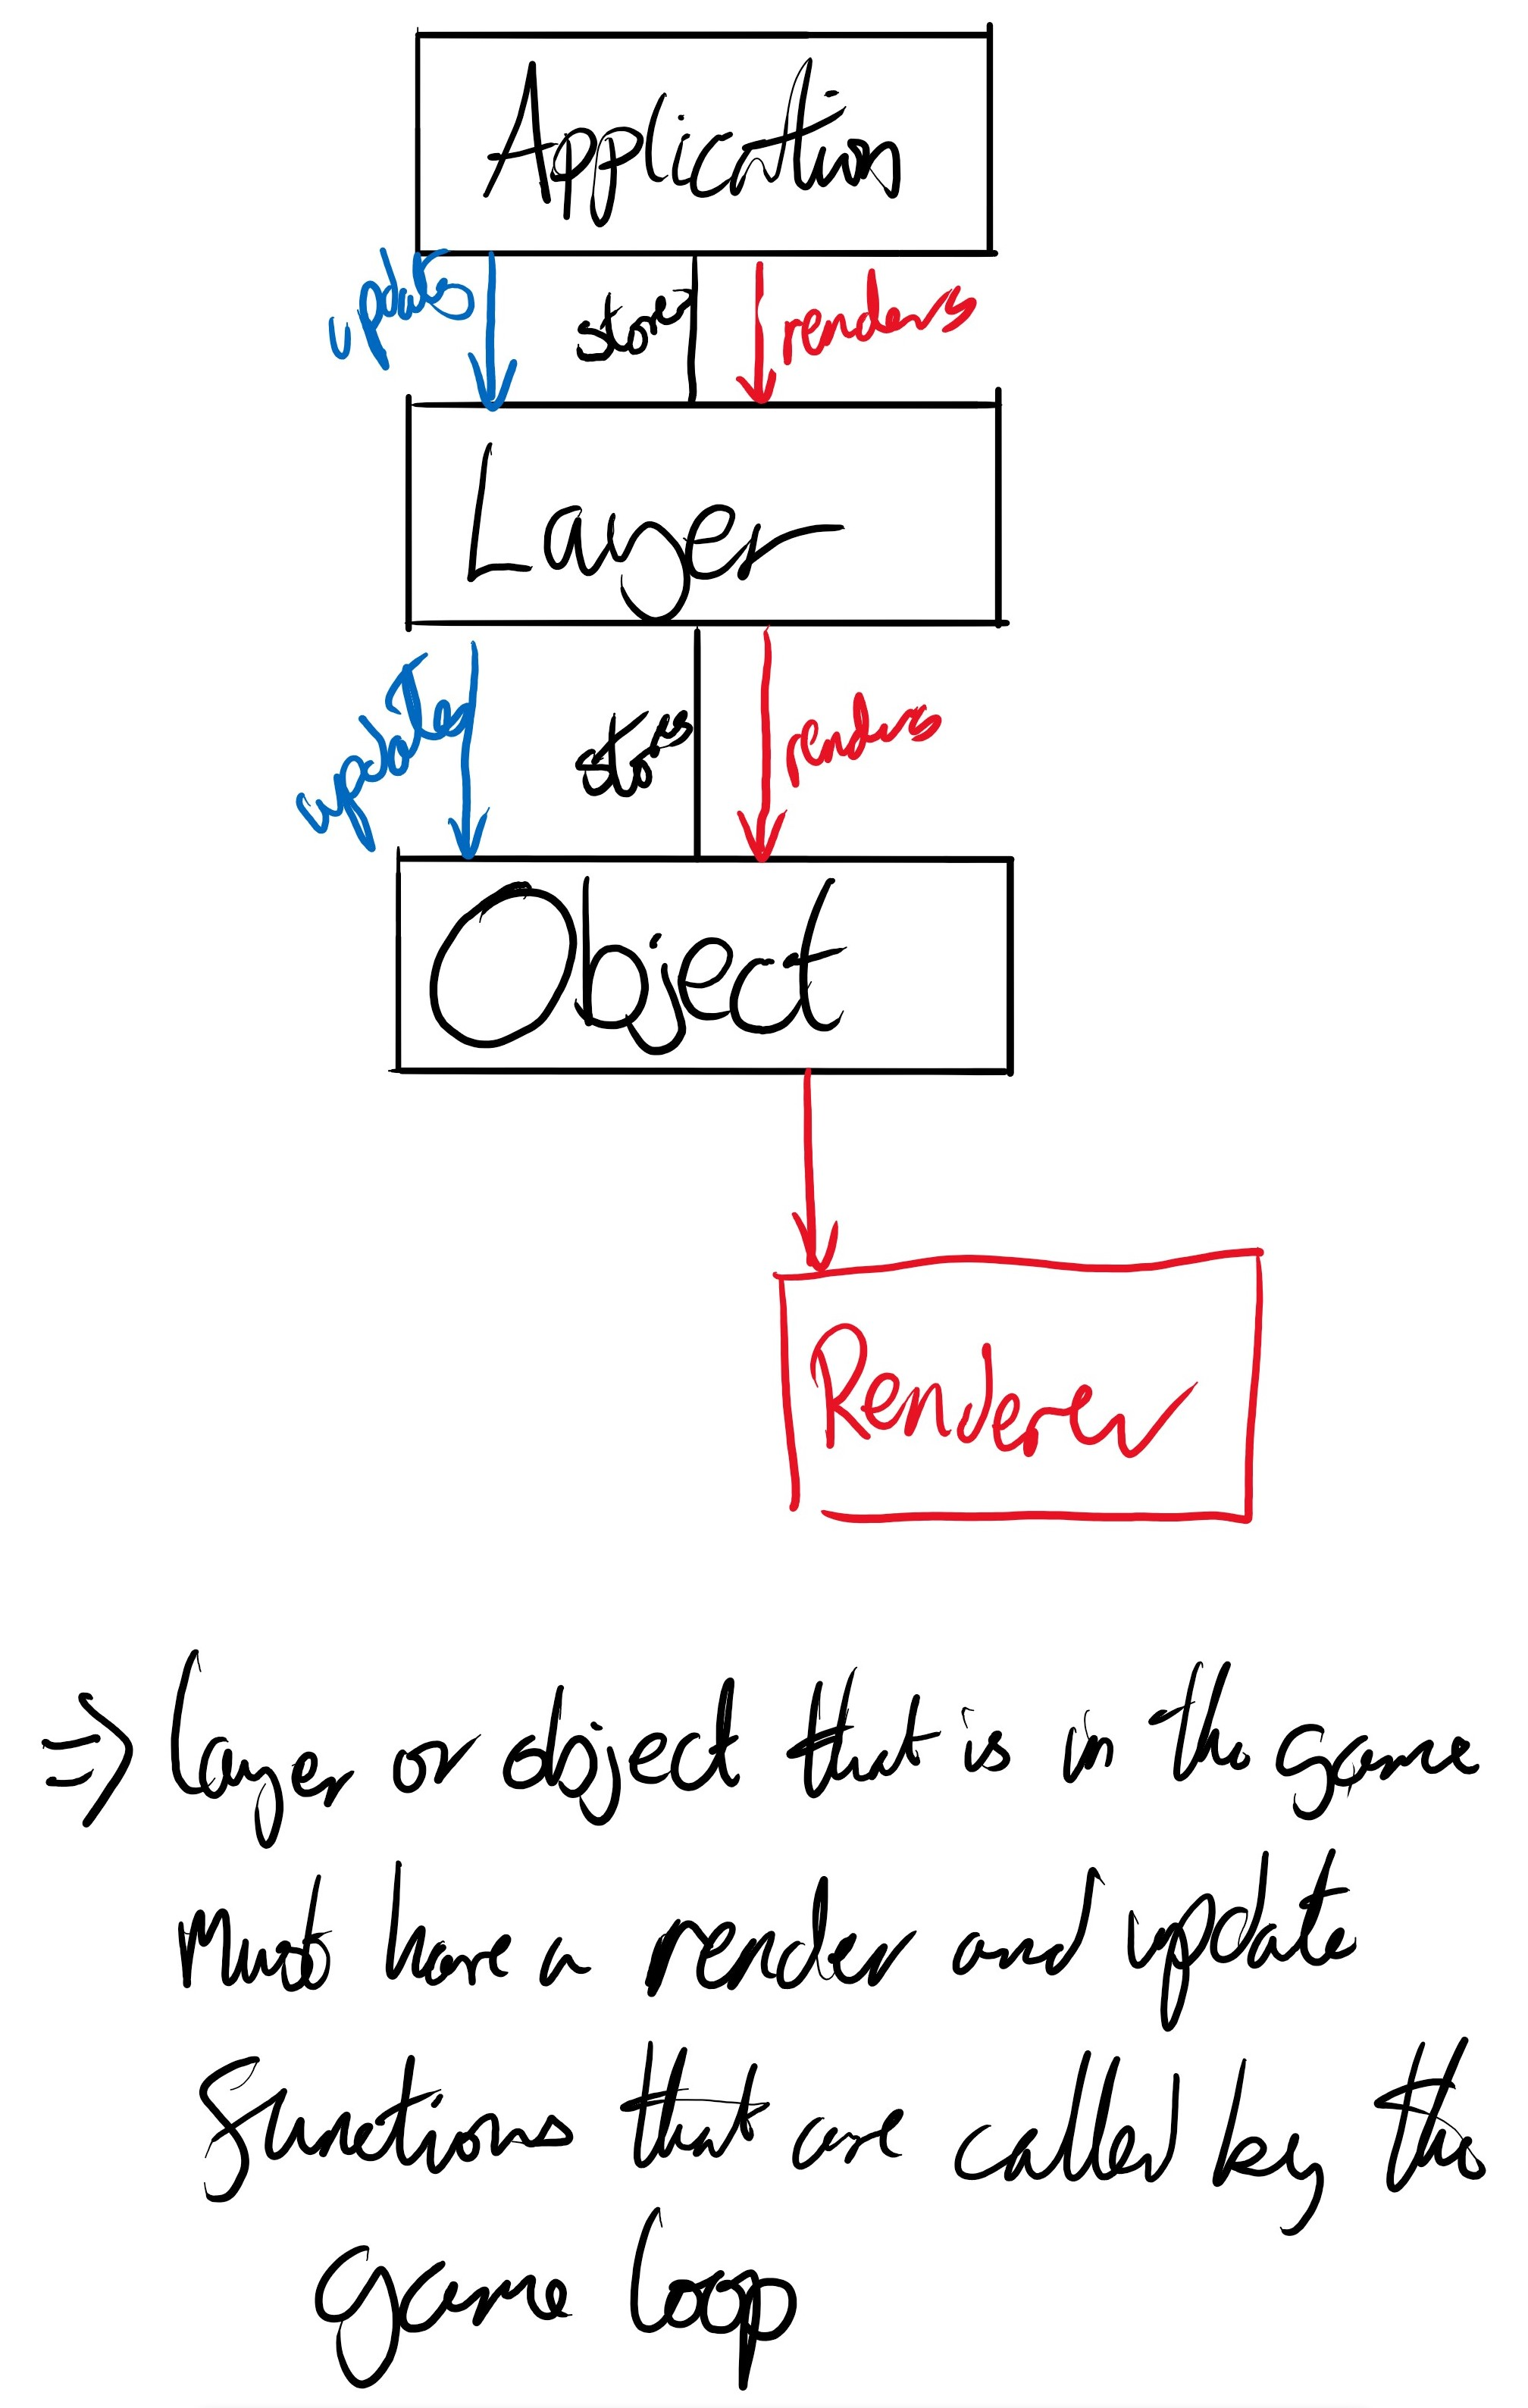
\includegraphics[scale=0.5]{img/Design/Struture.jpg}}
            \caption{Rough structure of the main principle of the application}
            \label{fig:Structure}
        \end{figure}
        As shown in Figure \ref{fig:Structure}, the application will store multiple layers (which could be a level). These layers will store objects (which includes entities, spawners, particles etc.). The application will control the rendering and updating through the gameloop. This game loop will call a render function (which should be in all layers) on every layer. These render functions should then call the render function in all objects on the objects that it stores on the layer. Then these objects will use the renderer (which will be a singleton) to render themselves on the screen.

        The same should happen for updating all the objects, the application should call the update function on the layer, which will then call the update function on all of its objects. This will allow a simple solution to the problem of how to render and update all the objects in the application. Furthermore, it will give the opportunity for the layer to determine what is rendered and updated.
    \subsection{Objectives}
        \begin{enumerate}
            \item Have an effective rendering system
                \begin{enumerate}
                    \item This system must use OpenGL - as it is the graphics library I am using for this project.
                    \item This means having a system in place where I can call a function, giving it a set of values, and then it will be automatically rendered, so that I do not have to deal with keeping track of how much of the buffer is used up
                    \item So once this is complete, I should have be able to render a tile, or multiple tiles on the screen.
                    \item Create a camera class that can move in the 2D plane with the keyboard.
                \end{enumerate}
            \item Be able to generate an infinite maze
                \begin{enumerate}
                    \item Add a room class that can generate the tiles for each location from reading a bitmap file.
                    \item This needs the rendering system to be finished, so that I can render the maze once generated.
                    \item The maze needs to be stored in effective means that means that it will not slow down everytime it generates more of the maze.
                    \item This needs to be able to generate a maze from nothing, with most of the board filled up.
                    \item Once this is in place, I can then make is so that once you can move in each direction and the maze will generate more of itself.
                    \item Create a class for the player, allowing them to be rendered into the maze and have the camera follow the player.
                \end{enumerate}
            \item Create NPCs that rome the maze and can start following you
                \begin{enumerate}
                    \item Create an NPC class that can be placed and rendered into the world.
                    \item Make it so that the follower can ask the level for the shortest route (which will use the A* algorithm).
                    \item Make it so that once they have the direction they need to go in, that they can move around the map.
                    \item Add different types of followers.
                \end{enumerate}
            \item Add items and a way to collect them with a simple space-based inventory system
                \begin{enumerate}
                    \item Add an inventory to each mob (player, follower, enemy)
                    \item Create an item class that can be found in the maze.
                    \item Allow the item to be picked up and put inside the inventory of the player
                    \item Make an inventory system, so that if the player has too much in their inventory they can chose what to get rid of.
                    \item Allow items to be passed to the followers (so that they act like storage for the player)
                \end{enumerate}
            \item Add combat into the game
                \begin{enumerate}
                    \item Add projectile class that can be created by the player and rendered onto the map.
                    \item Allow the projectile to move in the direction the player is facing, and when it collides with an entity or solid tile, it will delete itself.
                    \item Add a particle system, so that the projectile will produce particles with a solid colour, that will decay over time.
                    \item Adapt NPC class to allow for attacking (enemies will be NPCs that are attacking the player).
                    \item Add a health and other stats (strength, agility ...) for every mob (player, follower, enemy).
                    \item Make it so that when a projectile hits an entity it deals a random amount of damage (in a given range), and check if the entity has died or not. Create a system to deal with the player's death.
                    \item Create an algorithm for the enemies to attack the player and their followers, also allow the followers to use the same algorithm to attack the enemy
                    \item Allow the enemies to have followers, who also attack the player and their followers.
                    \item Add multiple weapons, which have different damages and particle effects.
                \end{enumerate}
            \item Create different rooms that can be found in the maze.
                \begin{enumerate}
                    \item Add multiple different rooms the player can find while exploring the maze.
                    \item This will include creating a chest that randomly generates items inside, which the player can pick up.
                    \item Update the maze generation slightly so that it can randomly generate the different types of rooms.
                \end{enumerate}
            \item Create a menu system
                \begin{enumerate}
                    \item Create a layer for handling GUI objects.
                    \item Create button objects that can run a function when clicked.
                    \item Overhaul the inventory menu to work with the new system.
                    \item Make the game updates to be paused when inside a menu.
                    \item Create a main menu, where you can start a new game.
                    \item Allow the user to get back to the main menu while playing the game.
                \end{enumerate}
            \item Finalise everything
                \begin{enumerate}
                    \item Add more stats to the mobs, which results in different effects to your damage and the number of followers you can have.
                    \item Add food into the game which acts like a potion and have random sprites generated.
                    \item Update the sprites of the maze so that it has a medieval theme.
                \end{enumerate}
        \end{enumerate}
\end{document}